% !TEX root = ./summary.tex

\section{Abstrakter Syntax Baum visualisieren}
\label{sec:visualizeAST}
Hier geht es darum den zu zeigen, wie man den Abstrakten Syntax Baum mithilfe von \antlr zu visualisieren. Im Folgenden wird der Abstrakter Syntax Baum als AST f"ur abstract syntax tree genutzt. 

\subsection{Vorgehen}
Den AST mithilfe von \antlr zu visualisieren ist ziemlich einfach. Man benutzt eine Hilfsklasse, die das f�r einen "ubernimmt. 

\begin{figure}[H]
	\centering
	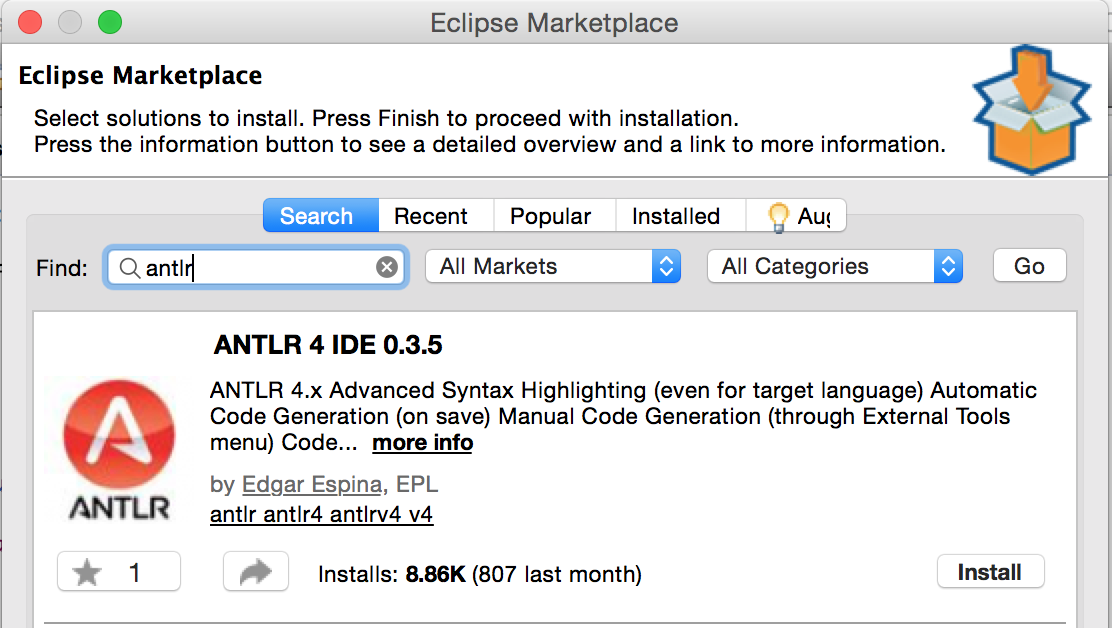
\includegraphics[width=0.65\textwidth]{antlr_plugin}
	\caption{Code um AST visualisieren}
\end{figure}